\section{Beer--Lambert depth profile in a metal}

The per-layer absorption returned by the TMM can be used to resolve the
spatial deposition of optical power with arbitrary resolution. This
benchmark slices a gold half-space into $N = 100$ virtual layers of
$dz = \SI{2}{\nano\metre}$ each, followed by a bulk gold half-space as
substrate, so the total thickness (\SI{200}{\nano\metre}) is deep enough
that the reflectance has converged to the bulk Fresnel value. The gold
refractive index at $\lambda = \SI{550}{\nano\metre}$ is taken from the
Johnson--Christy tabulation as $n_{\rm Au} = 0.425 + 2.367\,\ii$. Because
all $N$ slices carry the same index as the substrate, the slicing is a
pure reparametrisation of a continuous absorber.

With the field entering the metal at intensity $I_{\rm in} = 1 - R$ and
the absorption coefficient
$\alpha = 4\pi\,\Imy(n_{\rm Au})/\lambda$, the differential and
cumulative Beer--Lambert expressions are
\begin{align}
  \frac{\mathrm{d}A}{\mathrm{d}z} &= \alpha\,I_{\rm in}\,e^{-\alpha z}, \label{eq:bl-diff}\\[2pt]
  A(<z) &= I_{\rm in}\bigl(1 - e^{-\alpha z}\bigr). \label{eq:bl-cum}
\end{align}
Panel (a) compares the TMM per-layer absorption $A_j$, evaluated at the
midpoint depth $z_j = (j - 1/2)\,dz$, against
$\alpha\,dz\,(1 - R)\,e^{-\alpha z_j}$. Panel (b) overlays the cumulative
sum $\sum_{k \le j} A_k$ on the closed form~\eqref{eq:bl-cum}.

\begin{center}
\begin{tikzpicture}
  \fill[black!4] (0, 0) rectangle (5, 1.6);
  \foreach \i in {0,...,9} {
    \fill[yellow!40] (0,{-0.15*(\i+1)}) rectangle (5, {-0.15*\i});
    \draw[thin, gray!50] (0,{-0.15*\i}) -- (5,{-0.15*\i});
  }
  \fill[yellow!60] (0,-1.9) rectangle (5,-1.5);
  \draw[thick] (0,0) -- (5,0);
  \draw[thick] (0,-1.5) -- (5,-1.5);
  \node[lbl, anchor=east] at (4.9, 1.2) {air};
  \node[lbl, anchor=east] at (4.9,-0.75) {Au slices, $N \times dz$};
  \node[lbl, anchor=east] at (4.9,-1.7) {Au bulk};
  \raysketch{1.6}{0}{f}
\end{tikzpicture}
\end{center}

\begin{figure}[!htbp]
  \centering
  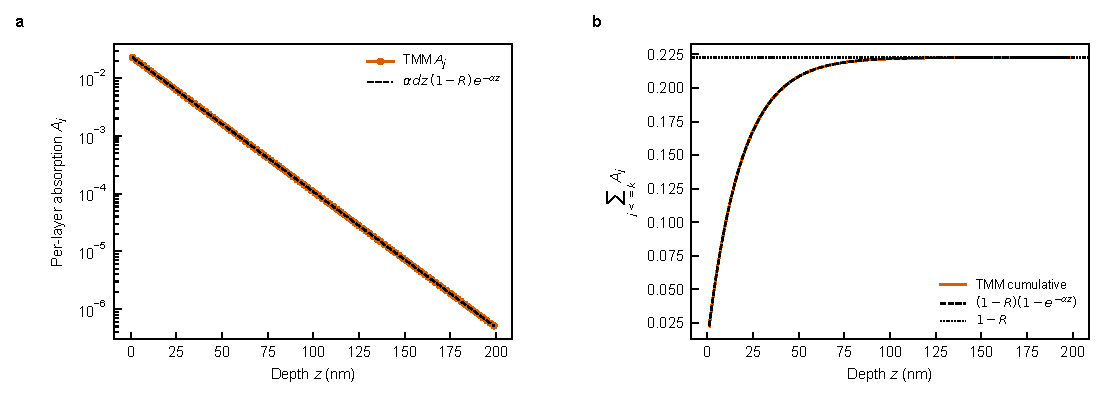
\includegraphics[width=\textwidth]{08_beer_lambert.pdf}
  \caption{(a) Per-layer absorption $A_j$ at slice midpoints, TMM versus the Beer--Lambert prediction. (b) Cumulative absorption up to depth $z$, TMM against the closed form~\eqref{eq:bl-cum}.}
  \label{fig:beer}
\end{figure}

The cumulative curve matches~\eqref{eq:bl-cum} to
$\max|A_{\rm cum,TMM} - A_{\rm cum,BL}| \approx \num{1e-15}$, which
confirms the total energy partition of the TMM. The differential
form~\eqref{eq:bl-diff} shows a residual of order $\num{5e-4}$ near the
surface; this is not a methodological bias but the finite-difference error
$\mathcal{O}(\alpha^{2}\,dz^{2})$ inherent to approximating
$\int_{z_j - dz/2}^{z_j + dz/2} e^{-\alpha z}\,\mathrm{d}z$ by the midpoint
value times $dz$. Halving the slice thickness to \SI{1}{\nano\metre}
reduces the residual to $\sim \num{1e-4}$, consistent with the quadratic
scaling.


